\documentclass[11pt]{article}
\usepackage[letterpaper,margin=0.85in]{geometry}
\usepackage[T1]{fontenc}
\usepackage{lmodern,microtype,amsmath,amssymb,booktabs,tabularx,graphicx,xcolor,enumitem}
\usepackage[hyphens]{url}
\usepackage{hyperref,fancyhdr}
\definecolor{navy}{HTML}{17324D}\definecolor{teal}{HTML}{176B73}
\hypersetup{colorlinks=true,linkcolor=navy,urlcolor=teal,pdftitle={Two-party private database: current estimate and historical MPC study}}
\setlength{\parindent}{0pt}\setlength{\parskip}{5pt}\setlength{\emergencystretch}{2em}
\setlist{nosep,leftmargin=1.5em}\setlength{\headheight}{14pt}
\pagestyle{fancy}\fancyhf{}\fancyhead[L]{\small\textcolor{navy}{Private database cost study}}
\fancyhead[R]{\small Conditional research estimate}\fancyfoot[C]{\thepage}
\newcommand{\F}{\mathbb F}
\begin{document}
{\color{teal}\large CURRENT TWO-PARTY PROPOSAL ESTIMATE}\par
{\color{navy}\LARGE\bfseries Garbled RAM and interactive Circuit OPRAM}\par
Updated 16 October 2026, America/New\_York\par
\textbf{Scope.} Two semi-honest parties; 10,000 flat key--value reads/s;
$N=2^{28}$ or $2^{32}$ records, 32-byte keys and 32-byte values, same-AZ
placement. Both cuckoo-table probes and both parties are included. The smaller
case is a padded planning size, not the exact 206.8M-account geometry. Merkle
proofs are outside this estimate. The ten-party analysis following these pages
is retained as historical research, not the current proposal recommendation.

\section{Current and proposed approaches}
\textbf{Current: two-party Garbled RAM. Proposed: streamed interactive 2PC
with Circuit OPRAM.} The proposed approach avoids retained future garbled
programs and exposes parallel work within a batch. Its resource estimate
remains conditional on a complete batch schedule and measured CPU/I/O rates.

\textbf{Routing review.} Only old leaf positions requested in the current batch
are opened, after duplicate masking. Sorting those positions and permuting the
associated wire labels is local work: no garbled sorting or Waksman circuit is
needed for a public permutation. Authorized final outputs, including selected
old child positions, can be decoded and reordered locally when the output
permutation is known. Secret results can also be rewired locally under a public
permutation. Live replacement positions remain hidden.

\textbf{Recomputed result: no additional gate discount from this change alone.}
The prior ledger did not separately charge public path ordering or terminal
output unpermutation. Its inverse-routing terms follow secret UID/destination
sorts and include private extraction/alignment allowances. They cannot all be
deleted as though they were public output permutations. A narrower extraction
or compaction circuit could reduce them, but has not yet been counted.

\begin{center}\small
\begin{tabularx}{\linewidth}{Xrr}\toprule
Interactive template, $B=256$, packing 8 & $N=2^{28}$ & $N=2^{32}$\\\midrule
AND gates / complete lookup (M) & 12.921 & 16.008 \\
Garbled tables / lookup (MB) & 413.5 & 512.3 \\
Network hosts per party & 546 & 676 \\
Network + SSD + modeled I/O (M USD/year) & 70.44 & 89.08 \\
With assumed 200M AND/s/node (M USD/year) & 83.28 & 104.97 \\
With assumed 50M AND/s/node (M USD/year) & 329.70 & 410.27 \\
\bottomrule\end{tabularx}\end{center}
All annual figures cover both parties and one state. The assumed CPU rates
include FreeXOR/runtime and utilization losses; neither rate is a benchmark.
The network/storage row omits CPU. Intra-party routing, complete initialization,
recovery and operational costs remain unpriced. These figures are planning
estimates, not proven upper/lower bounds or achieved service budgets.

\clearpage
\section{Which routing costs remain}
\begin{center}\small
\begin{tabularx}{\linewidth}{Xrr}\toprule
Retained private inverse-routing allowance (M AND/lookup) & $N=2^{28}$ & $N=2^{32}$\\\midrule
Private request conflict routing & 0.0660 & 0.0801 \\
Private pool result extraction/alignment & 0.9673 & 1.1748 \\
Private eviction routing/alignment & 2.2863 & 2.7768 \\
Private flat-map routing & 0.0004 & 0.0004 \\
Total retained inverse allowance & 3.3200 & 4.0321 \\
\bottomrule\end{tabularx}\end{center}
These amounts are \emph{subsets} of the total AND counts, not additional costs.
They are conservative composition allowances, not established minima. The
template does not establish that each resident record must return to its old
pool slot. Retaining a reordered pool may help, but output extraction and the
next state's invariants must then be specified and priced.

\paragraph{Why public paths do not determine the pool permutation.}
Pool lookup matches requested UIDs against hidden resident UIDs. After that
secret sort, the request rows occupy secret positions among resident records;
decoding the entire sorted array would expose unintended internal information.
Private extraction or compaction must produce the allowed outputs before local
reordering applies. Eviction selection depends on hidden destinations and
priorities, while cleanup hides real/dummy status. Distinct UIDs can share a
leaf, so equality of public paths cannot replace UID matching or deduplication.

\paragraph{Leading arithmetic.}
The three pool phases account for about 85--87\% of the current AND count.
With $A$ ANDs per lookup, half gates produce $32A$ bytes of tables. At
$R=10{,}000$ lookups/s, the per-party network count is
\[
 n_{\rm NIC}=\left\lceil\frac{1.05R(32A+\text{input bytes})}
 {7.9625\times10^9}\right\rceil,
 \qquad C_{\rm EC2}=2n_{\rm NIC}\cdot7.2576\cdot8760.
\]
The effective rate uses a 200-Gbps NIC with factors 0.65, 0.70 and 0.70.
The denominator is bytes/s; the multiplier 1.05 budgets framing. Prices retain
the October 12 AWS feed snapshot, refreshed unchanged on October 14; this is
not a new live price quote. The two roles are charged separately.

\paragraph{State count and latency remain conditional.}
For complete batch service time $L_B$ and batch size $B$,
\[
 S=\left\lceil\frac{10{,}000L_B}{0.70B}\right\rceil.
\]
One state at $B=256$ requires $L_B\le17.92$ ms. The mean batch-fill delay is
12.75 ms before queueing and service. Aggregate NIC/AND capacity does not prove
this latency. The $B=1024$ and $4096$ rows remain available in the JSON ledger;
no newly measured service time is implied by this routing review.

\clearpage
\section{Garbled RAM reference and next measurements}
The current-work comparison must enforce sequential evaluator service before
pricing independent states. Using the existing two-epoch retention model and
optimizing the horizon for each assumed service time gives:
\begin{center}\small
\begin{tabular}{lrrr}\toprule
Assumed complete lookup service & States & $N=2^{28}$ (B USD/year) & $N=2^{32}$ (B USD/year)\\\midrule
50 ms & 715 & 0.548 & 6.979 \\
100 ms & 1,429 & 0.991 & 13.563 \\
500 ms & 7,143 & 4.307 & 65.839 \\
\bottomrule\end{tabular}\end{center}
These cover network EC2, SSD capacity and attachment hosts, not full CPU,
SSD I/O or secure epoch renewal. Service times are assumptions, not Garbled
Merge measurements. The comparison does not establish an empirical savings
ratio or a universal Garbled RAM cost lower bound.

\paragraph{Next analysis.}
Specify a private output-extraction circuit that can retain pool order and
route only necessary result bits; validate packed-map updates and duplicate
handling. Then count its gates and live labels, benchmark both 2PC roles and
distributed batch service, and choose worker/replica counts from that service
time. Bucket capacity, pool slack and the service-lifetime overflow bound also
remain unresolved. Public-path routing is already removed from the secure
gate budget; treating it as a second discount would double-count the saving.

\paragraph{Reproduction.}
\begin{verbatim}
python -m mpc_cost.two_party_cost
python -m mpc_cost.two_party_serial
python -m unittest mpc_cost.test_two_party mpc_cost.test_garbled -v
python -m mpc_cost.render_report
python -m mpc_cost.render_short_report
\end{verbatim}
The routing decomposition is in
\texttt{results/two\_party\_comparison.json}; assumptions are in
\texttt{data/two\_party\_notes.txt}. The tests validate accounting, not a
complete implementation or security proof.

\paragraph{Primary references.}
Circuit OPRAM: \url{https://eprint.iacr.org/2016/1084};
half gates: \url{https://www.cs.virginia.edu/~evans/pubs/ec2015/};
Garbled Merge: \url{https://eprint.iacr.org/2026/761}.
The finite Boolean compilation and deployment assumptions are this study's
model, not measured results reported by those papers.

\clearpage
{\color{teal}\large HISTORICAL TEN-PARTY STUDY}\par
{\color{navy}\LARGE\bfseries A 10,000-query/s key--value database\\in ten-party honest-majority MPC}\par
Historical estimate dated 13 October 2026, America/New\_York\par
\textbf{Archive status.} The current proposal focuses on two parties, as
described in the opening sections. The following analysis preserves the
earlier ten-party investigation and its original assumptions. Its proposal
recommendations are superseded by the two-party scope.\par
\textbf{Target:} $2^{28}$ and $2^{32}$ records, 32-byte keys and values; ten parties, at most four
malicious corruptions, security with abort; average response time at most five seconds.

\textbf{Updated comparison.} The interactive reference costs approximately
\$2.33B/year and \$5.16B/year, respectively, at modeled mean latencies 4.77 and
3.97 seconds. Local arithmetic is the critical resource; RAM capacity also
constrains the larger case. Under the requested network-bottleneck assumption,
the conditional garbled-RAM model costs \$10.33--18.52B/year and \$21.59--38.71B/year using the
best prepared horizons in its grid. Preprocessing dominates its communication;
SSD retention is strongly horizon-dependent. Concrete correlation generation and
secure epoch renewal remain unpriced. Sections~\ref{sec:scale}
and~\ref{sec:garbled} give the calculations, sensitivities and limits.
The earlier detailed interactive sections use $N=2^{28}$ unless stated otherwise.

\section{Historical ten-party proposal decision}
\textbf{Continue with two cuckoo tables over binary Circuit OPRAM, but make the
arithmetic compilation and private routing the research contribution.} Probe both
tables in parallel; use a shared central batcher, grouped recursive-map updates,
private dot products, a larger flat base, and a sweep of position-map packing.
The important distinction is between increasing the number of labels per
recursive record and changing the ORAM tree's branching factor: this study changes
the former and retains the binary-tree eviction invariant.

\textbf{A low annual budget is not yet supported.} The explicit all-arithmetic
reference used here has millions of secure reduction outputs per logical read.
Its AWS sensitivity scenarios land in the billion-dollar/year range. That is a
warning about this compilation, not an impossibility result for the problem.
No complete malicious ten-party Circuit OPRAM benchmark or proof of these new
compiled circuits was produced. In particular, the model does not establish the
best achievable construction among mixed-domain, shuffle-based, hierarchical, or
other MPC memory protocols.

The useful budget milestone is to measure and reduce the complete per-read work
vector. A backend-conditional envelope below shows that even 10,000--30,000 secure
outputs per read can consume millions of dollars/year across ten parties. Those
counts are \emph{optimization targets}, not achieved costs of the proposed system.

\paragraph{Historical suggested proposal language (superseded).}
\begin{quote}
We will develop an honest-majority MPC key--value service using batched oblivious
access rather than a direct multiparty garbled-RAM extension. Our design combines
parallel cuckoo probes, arithmetic-aware recursive position maps, private inner
products, and optimized oblivious routing. We target 10,000 reads per second and
mean response time below five seconds. Preliminary circuit and cloud accounting
identifies metadata conversion and pool routing as the principal bottlenecks;
meeting a practical cost target requires reducing these costs. We will validate
throughput and annual operating costs with a complete malicious ten-party
implementation including preprocessing, maintenance, and all-party communication.
\end{quote}

\section{What the numerical search found}
The program searches batches 64--2048, fanouts 4--256, flat cutoffs 256--65536,
compact versus field-bit metadata, sorting networks versus a checked-shuffle
quicksort template, five EC2 instance sizes, and machines/replicas. It minimizes
EC2 expenditure among points with modeled mean latency below five seconds.
The cutoffs are requested limits; the actual flat map may be larger when another
recursive tree would be too small to support its parallel batch.

\begin{center}\small
\begin{tabular}{lrrrrr}\toprule
Scenario & Batch & Fanout & Actual base & \$/year (B) & Mean (s)\\\midrule
central & 128 & 128 & 32,768 & 2.33 & 4.77 \\
faster\_cpu & 128 & 128 & 32,768 & 1.52 & 4.65 \\
slower\_cpu & 128 & 128 & 32,768 & 6.06 & 2.92 \\
low\_exchange & 512 & 32 & 16,384 & 1.69 & 2.61 \\
slow\_exchange & 64 & 128 & 32,768 & 4.68 & 4.79 \\
two\_second\_target & 128 & 128 & 32,768 & 4.32 & 1.67 \\
no\_overlap & 128 & 128 & 32,768 & 3.96 & 4.56 \\
\bottomrule\end{tabular}\end{center}
These are independently optimized scenarios, not confidence intervals. The
two-second-target row tightens the mean-latency cap to two seconds
while retaining the central hardware assumptions. All other rows use five seconds.
The CPU
capacity assumptions are 0.5, 2, and 8 billion \emph{weighted} local field operations per
64-vCPU node/s. They are not measured EC2 performance. Exchange-delay assumptions
are 0.05, 0.2, and 0.5 ms; the central value is 0.2 ms. No-overlap sums CPU, network and RAM
service time; other rows take their maximum. The latency simulation assumes
Poisson arrivals and service-time coefficient of variation 0.05, and cannot predict
real network tails or failures.

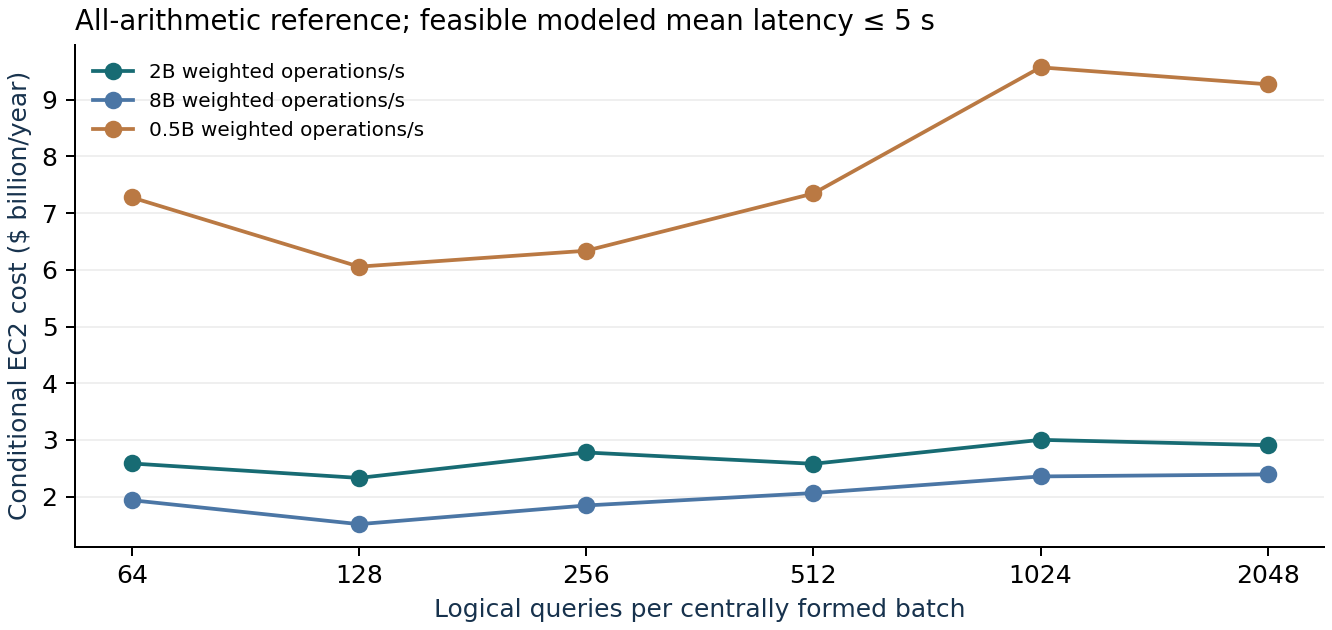
\includegraphics[width=\linewidth]{results/batch_cost.png}

The central minimum uses 128 queries, fanout 128, 32,768 scalar labels in each
flat base, and 3 recursive tree levels per cuckoo table. Its state occupies
1,926\,GiB per party per replica. It uses 6 machines per party per replica and
530 independent replica groups (31,800 machines across all parties).
Its modeled mean latency is 4.77\,s, of which 1.29\,s is dependent exchange time.
This enormous deployment is an accounting result, not a recommended AWS launch.
No EC2 capacity availability, quota increase, or linear scaling to this size has
been established.

\begin{center}\small\begin{tabular}{rrrrr}\toprule
Level & Records per table & Payload words & Pool records & Lower path buckets\\\midrule
0 & 536,870,912 & 6 & 893 & 22 \\
1 & 4,194,304 & 128 & 893 & 15 \\
2 & 32,768 & 128 & 893 & 8 \\
\bottomrule\end{tabular}\end{center}

Per logical read, this point charges 3.36 million reduction outputs,
182.2 thousand preprocessed random bits, and 629.2\,MB transmitted per party.
The byte count includes the leading backend costs and 5\% framing. Stored-field-bit
metadata reduces conversion work but expands persistent state to roughly 12--13\,TiB
per party for typical grid points. That is \emph{not} the memory cost of a properly
packed Boolean-sharing implementation; this model charges every bit as an
authenticated arithmetic share.

Fanout 128 wins the central scenario because it removes recursive levels; the
low-exchange scenario instead favors fanout 32. Thus neither ``largest payload''
nor ``smallest base'' is a robust optimum. For prototyping, test batches 128--1024,
fanouts 16, 32, 64, and 128, and actual bases of a few thousand to 32768 labels. Small batches
keep formation latency low; the model's several-second delay comes mainly from
computation and dependent communication, not waiting to fill batches.

\section{A cost envelope for optimization targets}
For $G$ scalar reductions or private-dot-product \emph{outputs} per read, the
leading SY-Shamir traffic proxy is
\[
 V_{\mathrm{party/read}}=G\cdot\frac{59}{6}\cdot16\ \text{bytes},\qquad
 V_{\mathrm{party/sec}}=10^4 V_{\mathrm{party/read}}.
\]
This excludes additional random bits, long-dot local work, conversions, routing,
and special openings unless they are charged separately. It is a conditional
backend relation, not an information-theoretic MPC lower bound.

\begin{center}\small\begin{tabular}{rrrr}\toprule
Outputs/read & Peak NIC floor & NIC + headroom & Assumed CPU + NIC\\
&\multicolumn{3}{c}{USD millions/year, all ten parties}\\\midrule
10,000 & 0.98 & 1.95 & 2.93 \\
30,000 & 1.95 & 4.89 & 8.80 \\
100,000 & 6.84 & 16.62 & 29.32 \\
1,000,000 & 61.57 & 159.31 & 290.28 \\
\bottomrule\end{tabular}\end{center}
The table uses \texttt{r6in.32xlarge}, 200 Gbps, \$11.15712/hour. Headroom includes
65\% NIC utilization, 70\% operating utilization, a 1.12 hottest-party factor, and
5\% framing. CPU+NIC assumes 83 weighted operations/scalar output and 2 billion
operations/s per 64 vCPU. It does not provision RAM, state replicas, dependent-round
latency, intraparty routing, failover, or database initialization. Consequently
even the rightmost column is not a sufficient deployment budget.

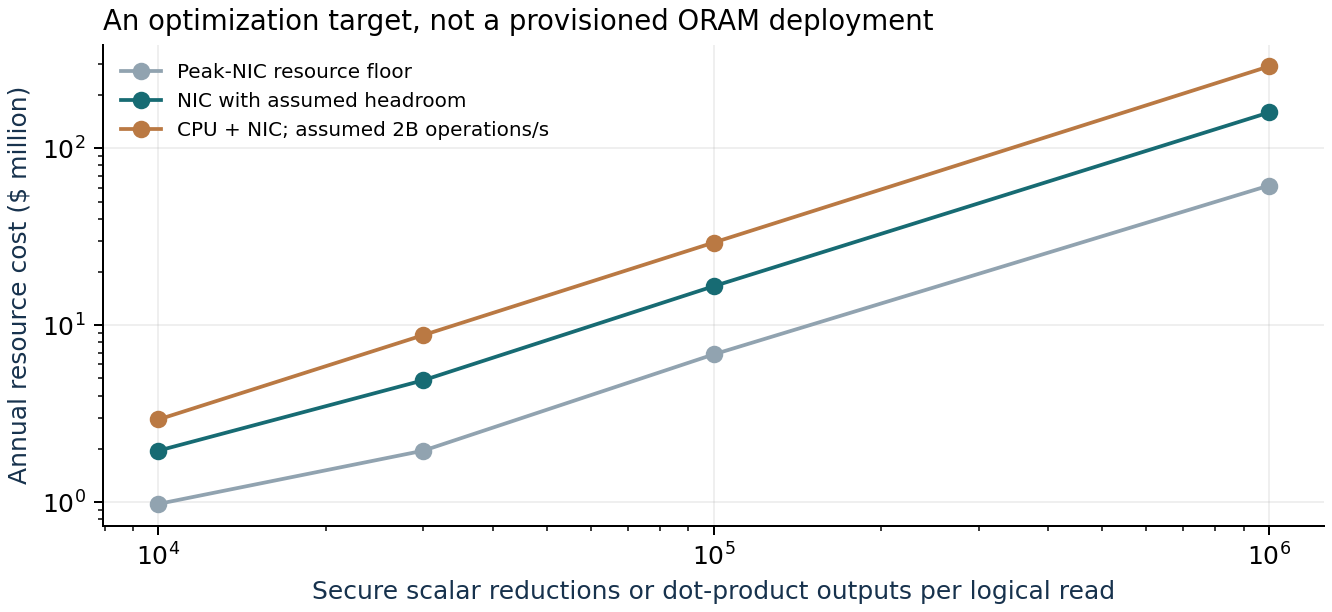
\includegraphics[width=\linewidth]{results/capacity_envelope.png}

The gap from the reference's roughly 3 million outputs/read to a 30,000-output
target is about 100-fold. Packing position maps alone cannot credibly be assigned
that improvement. A substantially different metadata/routing implementation is
needed before such a target can be presented as an expected system result.

\section{Backend and scheduling assumptions}
The accounting is tied to MP-SPDZ revision
\texttt{73eb8556cdfc670c5d3dc1067a3ae5b4ad0d4441}, using authenticated SY-Shamir,
$n=10,t=4,p=2^{127}-1$. The source-derived leading coefficient is approximately
$59/6$ field words sent per party per scalar/dot output; a checked opening costs
8 words, and an authenticated random bit about 24 words. A scalar multiplication
has one exchange; the current dot-product path has two sequential exchanges.
An active-check barrier adds at least four phases. Leading coefficients are not
complete measured wall-clock costs.\footnote{Pinned protocol source:
\url{https://github.com/data61/MP-SPDZ/tree/73eb8556cdfc670c5d3dc1067a3ae5b4ad0d4441/Protocols}.}

Keep these three kinds of arithmetic separate:
\begin{itemize}
\item One secret-selector payload mux uses one scalar product per field word.
\item A $k$-bit secret comparison uses a prefix circuit of about $3k-2$
products before its conditional movement; it is not one arithmetic gate.
\item An inner product of length$k$ has one communicated output but$\Theta(k)$
local arithmetic. Random bits and exact field-to-bit conversion require their
own preprocessing ledger.
\end{itemize}
The model's exact canonical-mask conversion and path-planning circuits have
explicit proxy coefficients. The mask acceptance work is charged offline;
conversion/opening phases are charged online. For a simple sustainable service
schedule, the batch resource time includes \emph{both} online and offline work.
Ready preprocessing and overlapped maintenance can lower online latency, but
their steady-state compute and network capacity must still be provisioned.

For $K$ machines per party in one replica, the capacity model uses
\[
 T_{\mathrm{service}}=D\tau+
 \max\{T_{\mathrm{network}},T_{\mathrm{CPU}},T_{\mathrm{RAM}}\},\qquad
 J=\left\lceil\frac{10^4T_{\mathrm{service}}}{0.7B}\right\rceil.
\]
$J$ is the number of independent evolving ORAM replicas. Each replica stores the
entire shared database; $K$ shards its physical state and computation. A 0.7
distributed-efficiency factor and explicit intraparty share-routing traffic
limit ideal scaling. The model adds scratch and a rough traffic-derived
preprocessing inventory proxy. An implementation must replace that proxy with
actual material sizes. The price is $10JKp_{\mathrm{hour}}\cdot8760$.

A central dispatcher forms a batch before choosing a replica. Mean formation
waiting is approximately $(B-1)/(2R)$: 6.35 ms at $B=128$ and 51.15 ms at $B=1024$.
Splitting arrivals into$J$ independent batchers would multiply that delay and is
not the deployment being priced. Every replica finishes maintenance before
accepting its next batch. The script also simulates dispatch queues, and tests
that inadequate service capacity causes queues to grow.

\section{AWS placement changes the answer}
The official Linux/shared-tenancy US East (N. Virginia) offer snapshot is
\texttt{20261012193925}, published 12 October 2026, with selected prices effective
1 October 2026. Raw rows and a refresh script are retained.\footnote{Official
offer feed: \url{https://pricing.us-east-1.amazonaws.com/offers/v1.0/aws/AmazonEC2/current/us-east-1/index.csv}.}

Same physical AZ VPC-peering traffic can avoid transfer fees, including across
accounts. Cross-AZ peering is\$0.01/GB at each endpoint, or\$0.02 for a transmitted
GB counted once.\footnote{\url{https://docs.aws.amazon.com/vpc/latest/peering/what-is-vpc-peering.html};
\url{https://aws.amazon.com/vpc/pricing/}.}
Thus at 10,000 outputs/read, the leading all-cross-AZ transfer bill alone is
\$99.2 million/year under this backend. For the central reference circuit it is
\$39.7 billion/year, before compute. A 4/3/3-party placement gives crossing fraction
$66/90$ only for uniformly weighted all-to-all communication; actual protocol
traffic needs a byte-weighted graph. AWS billing-unit assumptions are exposed.

Advertised NIC bandwidth is per direction; single-flow limits and multi-NIC
configuration matter. In particular, \texttt{r6in.32xlarge} needs both network
cards to attain the aggregate 200 Gbps. No sustained MPC bandwidth or collective
latency is guaranteed by the instance specification.\footnote{
\url{https://docs.aws.amazon.com/ec2/latest/UserGuide/ec2-instance-network-bandwidth.html};
\url{https://docs.aws.amazon.com/ec2/latest/instancetypes/mo.html}.}
The interactive prices exclude EBS, snapshots, setup, backups, client transfer, NAT,
orchestration, failover reserve, support, taxes, and engineering. Same-provider
or same-AZ placement does not by itself establish independent corruption domains.

% Design/research fragment. Included by the main cost report.
% No numerical cost conclusion is asserted by this fragment.
\section{Construction choice and what the estimates establish}

The design target is a read service for $N=2^{28}$ key--value pairs, each
containing a 32-byte key and a 32-byte value, at 10,000 logical requests per
second. The security target is ten parties with at most four malicious
corruptions and security with abort. Mean response time should remain below
five seconds, with lower latency preferred. The raw database is 16\,GiB;
cuckoo slack, tree buckets, shares, authentication, recursive maps, and
independent service replicas add to this substantially. Logical reads still
modify the ORAM's position maps and placement state. Application writes and
their replication protocol are outside this estimate.

The proposed starting point is two-choice cuckoo hashing over recursive
Circuit OPRAM, with both candidates probed on every lookup. Two separate
cuckoo tables permit two independent OPRAMs to run in parallel; this modestly
reduces individual pool sizes without requiring secret-dependent shard
routing. The model uses single-slot hashing with explicit slack and a scanned
overflow stash. Hash-table and ORAM stash capacities remain parameters that
need a failure analysis. If clients supply secret shares of indices computed
using public hash functions, the interface must specify which input
consistency properties are checked. A keyed hash evaluated inside MPC is a
different, additional cost; it has not been selected and is not implicitly
free.

\paragraph{Circuit OPRAM is more than a batch of Circuit ORAM paths.}
For $b$ probes into a binary tree with leaf depth $H$, let
$r=\lceil\log_2(2b)\rceil$. The parallel construction keeps disjoint subtrees
below depth $r$ and represents the upper tree and stash in a pool. Its
algorithms include private conflict resolution, pool retrieval, eviction
candidate selection, and pool cleanup. The deterministic eviction paths
occupy distinct subtrees. These are essential costs, not an optional
implementation detail.\footnote{Chan and Shi, \emph{Circuit OPRAM: Unifying
Statistically and Computationally Secure ORAMs and OPRAMs},
\url{https://eprint.iacr.org/2016/1084}.}

For accounting, the reference template uses
\[
 P=Z(2^r-1)+R_{\mathrm{stash}},\qquad h=H-r+1,
\]
where $Z$ is bucket capacity and $R_{\mathrm{stash}}$ is an exposed slack
parameter. A conservative temporary allocation allows $P+3b$ records while
fetched blocks and returned eviction candidates are processed. The pool
replaces the upper tree buckets; their storage must not be counted twice.
Recursion stops before an additional tree would have fewer than $2b$ leaves.
This capacity accounting does not certify the chosen concrete stash slack.

\paragraph{Reference compilation versus the best achievable system.}
The program constructs an explicit operation ledger for a plausible
Circuit-OPRAM-inspired compilation. It includes pool operations, metadata
conversion, record movement, duplicate handling, and eviction planning. Some
scan and planning coefficients are deliberately exposed estimates. It is
neither a complete circuit implementation nor a proven upper bound on every
implementation detail. Large reduction counts therefore demonstrate the
expense of this specified compilation; they are not a lower bound on MPC
lookup, a proof that the throughput goal is infeasible, or a claim to have
found the globally optimal construction. AWS prices translate these
conditional workloads into dollars; they do not validate the workload or
processor-throughput assumptions.

The accounting distinguishes scalar products, private inner-product outputs,
local arithmetic, random bits, openings, memory traffic, and dependent
communication phases. In an appropriate Shamir backend, an inner product
can communicate per output rather than per scalar term. Its local
computation still grows with its length. This distinction is particularly
valuable for retrieval and flat position-map bases.

\section{Optimizations with a concrete implementation path}

\paragraph{Use private shuffles to reduce repeated payload movement.}
The optimized reference sort augments each sorting key with a secret unique
ordinal, securely shuffles records, and then opens comparison outcomes.
Subsequent sorting moves are public local operations. The unique ordinal is
essential: otherwise duplicate-key comparison patterns can disclose
multiplicity. Vectorizing comparisons across quicksort recursion levels
exposes parallelism, although its height and latency remain random.
This shuffle-then-sort approach is described in the Orq implementation.
\footnote{\emph{Orq: Complex Analytics on Private Data with Strong Security
Guarantees}, SOSP 2025,
\url{https://cs-people.bu.edu/vkalavri/assets/pdf/orq-sosp25.pdf}.}

A generic realization has five fixed parties each choose a uniform private
permutation and input checked switching-network controls. Under static
corruption of at most four parties, at least one permutation remains hidden.
Uniform switch bits alone would not produce uniform permutations. Restoring
request order requires both undoing public sorting moves and applying the
secret networks in reverse; the latter is charged. This is a useful
reproducible baseline, but five sequential networks are expensive.

For a more ambitious implementation, benchmark a Shamir-specific permutation
primitive. The 2026 Shuffle2 work uses inner products and preprocessing to
obtain linear online shuffle communication in the malicious honest-majority
setting. Its published implementation measures semi-honest execution; the
paper's malicious overhead factors are estimates. Its offline cost also
remains substantial. Consequently, it motivates an optimization experiment,
not an unqualified replacement throughput assumption.\footnote{Gao et al.,
\emph{SLIDE: Shuffle Shamir Secret Shares Uniformly with Linear Online
Communication and Guaranteed Output Delivery}, especially Sections 5 and
Appendix C.4, \url{https://arxiv.org/html/2608.27129v1}.
Implementation: \url{https://github.com/GJCPP/ShamirShuffle}.}

\paragraph{Specialize pool operations rather than sorting everything alike.}
Pool cleanup is stable compaction on validity bits. Local prefix sums and
scalar products can compute a unique secret destination permutation, leaving
private routing as the expensive primitive; long-key comparisons are
unnecessary. Maintaining the pool in logical-address order also permits a
derived finite-difference gather: attach differences of adjacent payloads to
pool records, insert zero increments for requests, merge by address, and use
local prefix sums to recover candidate values. Secret equality still decides
whether an exact match exists. Candidate-selection routing must subsequently
be undone and stable compaction must preserve the sorted-pool invariant.
This optimization needs an implemented invariant check and security argument;
it is not assumed by the reference scan coefficients.

\paragraph{Choose metadata representation separately from payload encoding.}
Moving one field word and comparing a secret integer have different costs.
Repeatedly converting compact arithmetic metadata to bits is expensive;
retaining every address and leaf bit as an arithmetic share expands both
storage and routing. A practical comparison should include compact metadata,
retained bit metadata, and a mixed representation with narrow comparisons
and explicit conversion costs. Retained bits must be charged whenever their
record moves. Leaf compatibility against a public eviction path can reuse
prefix-match products; target-depth comparisons use roughly $\log_2 H$ bits,
rather than the full key width.

The published depth analysis of Circuit ORAM provides a starting point for
parallel eviction planning. Its word-depth bound is not directly an MPC-round
bound: comparison, selection, and authentication phases remain to be
compiled.\footnote{Chan, Chung, and Shi, \emph{On the Depth of Oblivious
Parallel RAM}, \url{https://eprint.iacr.org/2017/861}.}

\paragraph{Tune recursive packing and the base together.}
Packing $F$ parent labels per recursive block reduces record counts but
increases record width, private subblock selection, and routing cost.
Moderate powers of two, for example $F=8$ through $128$, are useful search
points rather than a predetermined optimum. The binary eviction tree can
remain unchanged. Several requests may update different offsets of the same
map block: group those updates privately and commit the block once.
Independent whole-block writes would overwrite each other.

The base contains one scalar label per record in the last instantiated tree.
It is not smaller by another factor of $F$ unless another recursive tree has
been paid for. With $n=2^d$ base labels, a divide-and-conquer one-hot decoder
has the derived multiplication recurrence
\[
 T(d)=T(\lfloor d/2\rfloor)+T(\lceil d/2\rceil)+2^d,
 \qquad T(0)=T(1)=0,
\]
and depth $\lceil\log_2 d\rceil$. For $n=4096$, this is 4,272 products per
request and four product layers, before validity gating and read/write
operations. After duplicate resolution, dot-product retrieval and aggregated
updates need about $b+n$ reduction outputs, while local work remains
proportional to $bn$. Compare this against a complete additional recursive
level. The reference program uses the divide-and-conquer decoder, adding one
product and a conservative extra phase for a secret representative-valid bit.

\paragraph{Optimize scheduling after retaining dependencies.}
At one level, pool fetch and subtree fetch can overlap once old labels are
available. Maintenance on an already accessed recursive tree can overlap
fetching from the next tree if remapping labels have been sampled beforehand
and state updates are coordinated. Recursion still has a base-to-data fetch
dependency, and the next batch must not observe an uncommitted state. A sum
of all phase counts is a conservative serial schedule; replacing it by the
maximum level depth would be unjustified. Centrally forming batches before
dispatching them to independent replicas avoids multiplying formation delay
by the number of replicas. At 10,000 requests/s, batch size $Q$ alone adds
approximately $(Q-1)/(2\cdot10{,}000)$ seconds of mean formation delay.

\section{Validation needed before using a deployment budget}

The next experiment should implement and measure one complete recursive
batch, including duplicates and misses, on the selected malicious backend.
Separately measure comparison/conversion, shuffle and inverse routing, pool
cleanup, subblock updates, eviction, and preprocessing replenishment. Then
measure the composed dependency schedule and memory footprint, rather than
inferring end-to-end performance from multiplication throughput alone.

Failure parameters must cover the intended deployment lifetime. One year at
10,000 requests/s contains about $2^{38.2}$ logical requests, before counting
two probes, recursive levels, replicas, and checking events. If $A$ events
each have failure probability at most $\epsilon$, a simple lifetime bound is
$A\epsilon$. For example, an annual target of $2^{-40}$ with $2^{42}$
relevant events would require per-event probability at most $2^{-82}$.
The ORAM stash, cuckoo overflow, statistical checks, and any randomized
sorting limits need their own justified bounds. A simulated absence of
overflow is useful testing evidence but does not establish such a bound.

Finally, capacity should include authentication and preprocessing, local
routing between machines of one party, batch queues, and the full memory of
each independently evolving replica. Cross-availability-zone placement
changes both communication charges and latency. The resulting estimate is a
proposal-planning scenario until an end-to-end malicious implementation has
been calibrated on the intended topology.



\clearpage
\section{Bottleneck clarification and scan comparison (13 October update)}
\label{sec:bottleneck}
\textbf{The current model is limited first by total CPU demand, then by online
communication. Storage is large, but is not the binding constraint at the selected
point.} This is a diagnosis of the analytical model, not a measured profile of an
implemented MPC service. The earlier report combined online and preprocessing
work; the new ledger separates them without changing its total costs.

For the selected 128-query batch on six \texttt{r6in.24xlarge} machines per party:
\begin{center}\begin{tabular}{lr}\toprule
Resource or dependency & Time per batch\\\midrule
CPU, including preprocessing & 3.452 s\\
Network, including preprocessing and internal routing & 2.225 s\\
Modeled RAM traffic & 0.094 s\\
Dependent exchanges & 1.291 s\\\midrule
Service time: $1.291+\max(3.452,2.225,0.094)$ & 4.743 s\\
\bottomrule\end{tabular}\end{center}
These resource times are not additive under the model's overlap assumption.
Total mean response time is about 4.77 s after batch formation and fixed response
overhead. Faster CPUs eventually make networking or round latency dominant.

\subsection{What is offline and what is online?}
The selected SY-Shamir backend does not consume one Beaver triple per scalar
multiplication. Its main product/degree-reduction traffic depends on the live
inputs. Preprocessing supplies fresh checking randomness, random bits, and
canonical masks. Thus importing a triple-generation bottleneck from a different
SPDZ backend would misdiagnose this model.

\begin{center}\begin{tabular}{lrrr}\toprule
Per party, per logical read & Preprocessing & Online & Total\\\midrule
Sent traffic, decimal MB & 148.0 & 481.1 & 629.2\\
CPU proxy, million weighted operations & 122.9 & 216.9 & 339.8\\
\bottomrule\end{tabular}\end{center}
The traffic includes 5\% framing, counts each send once, and excludes intraparty
redistribution. CPU units are weighted source-operation estimates, not measured
cycles or seconds. All ten parties incur the corresponding resource demand.

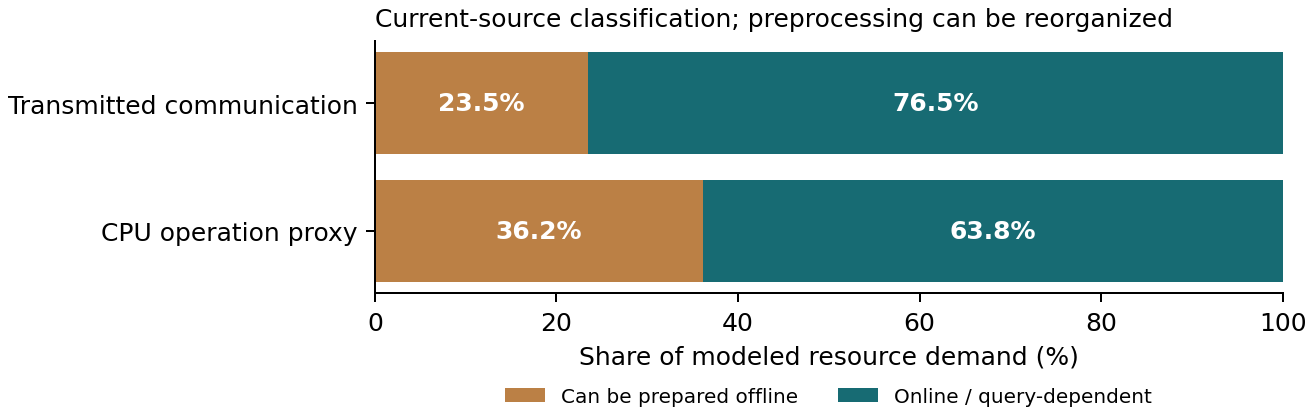
\includegraphics[width=\linewidth]{results/online_offline_breakdown.png}

For $O$ scalar/dot outputs, $C$ canonical masks, and $B_r$ random bits, the leading
preprocessing allocation is
\begin{align*}
 W_{\rm off}&=\tfrac56O+9(126C)+24B_r+8C,\\
 A_{\rm off}&=15O+68(126C)+330B_r+35C.
\end{align*}
$W$ counts transmitted field words per party; $A$ is the local CPU proxy. A full
output costs $9+5/6$ words: 9 for query-dependent resharing and 5/6 for a fresh secret
checking coefficient. Mask acceptance uses 126 outputs and an opening offline.
Fixed checks add small terms retained in the program. The online column is the
unchanged total minus this allocation.\footnote{Source accounting is pinned to
MP-SPDZ commit \texttt{73eb8556cdfc670c5d3dc1067a3ae5b4ad0d4441}; see
\url{https://github.com/data61/MP-SPDZ/tree/73eb8556cdfc670c5d3dc1067a3ae5b4ad0d4441/Protocols}
and the local ledger \texttt{data/mpc\_sources.txt}. These are derived counts,
not an official benchmark table.}

\textbf{The CPU phase boundary can move.} Precomputing random polynomial
contributions to scalar resharing can shift another 48 operations per live scalar
output out of the online loop. In this sensitivity, preprocessing rises from
36.2\% to about 81.1\% of total CPU work, with unchanged steady-state arithmetic.
This requires additional material storage, memory traffic, and a correct scheduling
implementation. It does not make that computation or its dollar cost disappear.
The 9-word live communication remains query-dependent. Likewise, ready preprocessing
can improve response time even when the service's sustainable throughput is still
limited by generating it. The existing 4.74 s service estimate charges full resource
production per batch; it is not an online-only latency benchmark.

\subsection{Storage and replication}
The selected state is 1,926 GiB (1.88 TiB) per party per ORAM replica, or about 2,217 GiB
including the modeled scratch/reserve. At 75\% usable memory, each 768 GiB instance
provides 576 GiB, so four machines suffice for capacity. Six are selected to meet
the latency/throughput model. Removing the memory constraint and re-searching the
same instance size leaves the selected price unchanged. Storage would become
binding under another representation or scheduling policy; field-bit metadata
in particular expands it substantially.

The previous \$2.33B/year deployment dedicates machines to each of 530 independently
evolving ORAM states. An asynchronous scheduler could share machines across those
states during round waits. The aggregate CPU-capacity requirement is 2,312 machines
per party (about \$1.69B/year), and their aggregate RAM could hold those 530 states.
That is a resource-capacity estimate, not proof that a scheduler achieves the
latency bound. The extra dedicated-instance cost is not an inherent cryptographic
lower bound. Do not allocate VM dollars proportionally to the CPU/traffic percentages:
one fleet serves overlapping demands.

\subsection{Naive parallel full-key scan}
The direct baseline compares every query key with all $N=2^{28}$ stored keys,
then returns $\sum_i [k_i=q]v_i$. Comparisons run in parallel across rows and queries;
rows are visited in a public order. Values use three private dot products, so their
selection communicates per output, not per record. There is no ORAM maintenance.
The dictionary has unique keys; the sum of match bits gives a private hit indicator.

The baseline uses \emph{exact} equality optimized for this field.
Represent a key with the same three field limbs as the ORAM. Since
$p=2^{127}-1\equiv3\pmod4$, $-1$ is a quadratic nonresidue and
$a^2+b^2=0$ holds exactly when both inputs are zero. For limb differences $d_0,d_1,d_2$,
compute
\[
 u=d_0^2+d_1^2,\qquad v=u^2+d_2^2,\qquad e=1-v^{p-1}.
\]
Each sum of squares is a length-two private dot product with one reduced output;
the 135-product exponentiation is the addition-chain routine from the model.
Thus each comparison costs 137 secure outputs, versus 407 for independently
zero-testing and combining three limbs. This equality also improves the ORAM's
few final key checks, but changes its millions-of-outputs total by less than 0.1\%.
Intermediate dot results must be degree-reduced before reuse.

Ignoring the tiny shared frontend, the full scan requires
\[
 G_{\rm scan}=137N+3\simeq36.8\ \text{billion outputs/read}.
\]
Batching does \emph{not} divide this count by batch size: a batch has $137NB$
comparison outputs. It reduces communication scheduling overhead and permits
database-cache reuse. Use row/query tiling, not an $N\times B$ materialized equality
matrix. The read-only 48 GiB of authenticated database shares per party can be shared
across concurrent workers, unlike independent mutable ORAM placements.

\subsection{An indexed alternative using private dot products}
An indexed scan is another baseline: keep the same two cuckoo tables
and scan their arrays without ORAM. Private dot products allow a two-dimensional
read. Arrange each $D=2^{29}$-cell table as an $A\times C$ matrix, with $AC=D$.
For private row and column one-hot vectors $a,b$, compute, for each payload word,
\[
 z_i=\sum_j b_jX_{ij},\qquad y=\sum_i a_i z_i.
\]
This reads every cell through local arithmetic, but only $AW+W$ dot outputs are
reduced. With $W=6$ key/value words, communication is minimized near
$A=\sqrt{D/(W+1)}$. The model chooses $A=8192,C=65536$. One-hot generation is charged,
both tables are always probed, and full keys plus the cuckoo stash are checked
exactly. Empty-cell validity can use an unused bit in the last key limb, so the
six-word payload need not grow. This is a derived exact read construction; it
does not imply a fast write protocol.

Its approximately 249,000 outputs/read are \emph{fewer} than the ORAM reference,
but its dot products still process both full arrays. The current source proxy
charges approximately $4\cdot2DW=25.77$ billion local operations/read before the
small remaining costs. Packing the batch as matrix multiplication can change
the actual cycles/operation; this must be measured independently. Our CPU-rate
assumption is not a benchmark of that dense kernel. Both scan variants can pipeline
queries and reuse immutable shares without paying for one full state per worker.

\subsection{Side-by-side work and cost}
\begin{center}\small\begin{tabular}{lrrr}\toprule
Per logical read / party & OPRAM & Full-key scan & Indexed 2D scan\\\midrule
Secure outputs & 3.36M & 36.78B & 0.249M\\
Local CPU proxy & 0.340B & 3,059B & 25.79B\\
Sent bytes, including framing & 629MB & 6.08TB & 41.2MB\\
Persistent shares & 1,926GiB & 48GiB & 192GiB\\
Exchange-depth contribution & 1.291s & 0.030s & 0.031s\\\bottomrule
\end{tabular}\end{center}
Storage is per complete state per party, not per read. Exchange-depth figures
are only the phase-delay term at 0.2 ms/exchange; they are not achievable response
latencies without sufficient computation and networking. Memory traffic is
optimistically tiled/reused for scans; detailed scratch and reduction aggregation
are not claimed to be free in an implementation.

Under the \emph{same unmeasured} 2-billion-weighted-operations/s per 64-vCPU assumption,
the common aggregate resource-capacity calculation gives:
\begin{center}\begin{tabular}{lr}\toprule
Construction & Annual resource equivalent, ten parties\\\midrule
OPRAM reference & \$1.69 billion\\
Naive full-key scan & \$15.25 trillion\\
Indexed 2D dot scan & \$128.6 billion\\\bottomrule\end{tabular}\end{center}
These all use \texttt{r6in.24xlarge} at the same 12 October price snapshot, 70\%
distributed efficiency and 70\% utilization. They are not new deployment quotes.
The scan fleets are astronomically large extrapolations, not plausible AWS
reservations. The common calculation excludes detailed sharded-dot aggregation,
queue/SLA feasibility, setup and scratch provisioning; its purpose is to expose
the scale of work. The previous \$2.33B ORAM figure includes a particular dedicated
replica policy and should not be compared with a CPU-only scan calculation as
if both were equally complete deployments.

Relative to the OPRAM reference, the naive scan needs about 9,000 times the CPU
proxy and 9,656 times the traffic. The stronger indexed scan needs about 76 times
the CPU proxy but only 6.5\% of the traffic. Therefore ``scan is communication-heavy''
is true for the naive full-key implementation, but false as a universal statement.

\paragraph{Practical conclusion.}
The next measurements should isolate (1) total preprocessing production,
(2) live product/resharing throughput, (3) checked network exchanges and
(4) a batched local matrix-contraction kernel. The current arithmetic OPRAM
reference uses less modeled CPU work than these scans, while the two-dimensional scan is
a serious bandwidth-oriented comparator. Neither the numerical CPU split nor
the cheapest real system is settled without those measurements.

Reproduce the comparison with \texttt{python -m mpc\_cost.compare\_scans};
the complete ledger is \texttt{results/bottleneck\_scan\_comparison.json}.



\clearpage
\section{Scaling the interactive MPC service to \texorpdfstring{$2^{32}$}{2 to the 32} records}
\label{sec:scale}
The larger proposal case retains 32-byte keys, 32-byte values, ten parties,
four malicious corruptions with abort, and 10,000 logical reads/s. We repeat the
complete parameter sweep and its CPU/exchange sensitivities. Both cases use two
cuckoo arrays whose combined capacity is $4N$ at the rounded 40\% load ceiling;
the actual occupancy is 25\%. These estimates cover flat key/value lookups, not
Merkle-proof retrieval. The $2^{28}$ case is a power-of-two planning size, not the
proposal's exact 206.8-million-account count.

\begin{center}\small\begin{tabular}{lrr}\toprule
Selected central reference & Smaller database & Larger database\\\midrule
Logical records & $2^{28}$ & $2^{32}$ \\
Raw key/value database & 16 GiB & 256 GiB \\
Batch / map packing fanout & 128 / 128 & 512 / 256 \\
Actual flat base (labels/table) & 32,768 & 131,072 \\
Recursive ORAM trees/table & 3 & 3 \\
Secure outputs/read & 3.36M & 6.10M \\
Sent MB/read/party & 629.2 & 1,085.8 \\
State TiB/party/replica & 1.88 & 30.05 \\
Nodes/party/replica & 6 & 96 \\
Independent replicas & 530 & 110 \\
All-party EC2 instances & 31,800 & 105,600 \\
Modeled mean latency & 4.77 s & 3.97 s \\
Conditional EC2 USD/year & \$2.33B & \$5.16B \\
\bottomrule\end{tabular}\end{center}
The smaller selection uses \texttt{r6in.24xlarge}; the larger uses
\texttt{r6in.16xlarge}. Prices, throughput assumptions and the 5-second mean
limit are unchanged. The full search includes batches 64--2048, fanouts 4--256,
both metadata representations and both sorting templates. The larger selection is on the upper fanout boundary; it is the best point in this grid, not a global optimum.
The flat base contains 131,072 labels despite a nominal cutoff of 256, because the next tree would have fewer than $2B$ leaves. The model stops recursion there.
The complete sensitivity runs are saved in \texttt{results/size\_2p32/}.

\textbf{The bottleneck changes with size.} For the $2^{32}$ selection, CPU demand
is 2.180 s/batch, network demand is 1.595 s and dependent exchanges
add 1.742 s. CPU still controls the resource term, but RAM capacity also
constrains provisioning: the state plus modeled scratch/buffer requires 34.57
TiB per party per replica. Each selected 512-GiB instance provides 384 GiB of
usable RAM, requiring at least 93 nodes; the grid selects 96. At the same fixed
circuit and instance type, removing only the memory constraint gives 66 nodes,
138 replicas and approximately \$4.45 B/year. Thus the earlier statement
that storage does not affect the chosen fleet applies to the $2^{28}$ reference.

Per $2^{32}$ logical read and party, preprocessing accounts for 192.1 MB and
168.1 million weighted CPU operations; online work accounts for 893.7 MB and
404.2 million operations. These are the same source-derived phase allocations
as Section~\ref{sec:bottleneck}, not new measured rates. The selected mean is lower than in the
smaller case because memory capacity forces a larger parallel allocation, not
because larger databases inherently have lower latency.

\subsection{Scan comparison at both sizes}
\begin{center}\small\begin{tabular}{llrrr}\toprule
Records & Construction & Weighted Gops/read & GB sent/read & USD B/year\\
&&\multicolumn{2}{c}{per party}&all parties\\\midrule
$2^{28}$ & OPRAM & 0.34 & 0.629 & 1.69 \\
$2^{28}$ & Full-key scan & 3,058.82 & 6,075.355 & 15,252.97 \\
$2^{28}$ & Indexed 2D scan & 25.79 & 0.041 & 128.61 \\
$2^{32}$ & OPRAM & 0.57 & 1.086 & 2.85 \\
$2^{32}$ & Full-key scan & 48,941.15 & 97,205.683 & 244,047.48 \\
$2^{32}$ & Indexed 2D scan & 412.40 & 0.163 & 2,056.45 \\
\bottomrule\end{tabular}\end{center}
The last column uses the common aggregate resource-capacity model from Section~\ref{sec:bottleneck};
it does not include a latency-feasible replica schedule. In particular, its ORAM
figures differ from the dedicated-replica costs above. Scan state remains shared
across concurrent read workers: at $2^{32}$, it is 768 GiB/party for full-key
scanning and 3,072 GiB/party for the indexed two-array scan. Full scanning grows
almost exactly 16-fold in computation and traffic. Indexed scanning grows about
16-fold in local work and fourfold in transmitted data because of the balanced
two-dimensional layout. All figures still depend on unmeasured CPU rates.



\section{Multiparty garbled RAM: both database sizes}
\label{sec:garbled}
\textbf{Under the requested communication-bottleneck assumption, recurring
garbling preprocessing is the main traffic cost.} About 97.7\% of modeled bytes
are preprocessing, not the delivered garbled tables. SSD capacity can nevertheless
dominate the dollar bill if a long future execution is retained in full. The
reference policy below costs \$10.33--18.52B/year at $2^{28}$ records and
\$55.07--65.69B/year at $2^{32}$. Shortening the latter's prepared horizon reduces the
conditional estimate substantially. None of these ranges includes a measured,
finite OT-only correlation generator or a complete malicious epoch-renewal protocol.

\subsection{Scope and Boolean work ledger}
We use \emph{Multiparty Garbling from OT with Linear Scaling and RAM Support}
(ePrint 2025/444), including Appendix H and its tri-state encoding in Appendix F.
The local 49-page PDF was checked directly. The ten-party setting tolerates four
static malicious corruptions with abort. Field elements and labels have width
128 bits; this is a parameter choice, not a demonstrated 128-bit service-lifetime
failure bound.\footnote{\url{https://eprint.iacr.org/2025/444}. The retained local
source is \texttt{multiparty\_ot.pdf}; detailed equation notes are in
\texttt{data/garbling\_backend\_notes.txt}.}

As requested, all garbled-stack and associated adaptor costs are set to zero,
assuming the two-party improvement in ePrint 2026/761 can be migrated. That paper
optimizes the stack subroutine; it does not remove ordinary RAM reads, eviction,
recursive maps, or initialization. Its measured regime is two-party, up to
$2^{24}$ cells. Our extrapolation is consequently a conditional multiparty
construction, not a published benchmark.\footnote{\url{https://eprint.iacr.org/2026/761},
local \texttt{garbled\_merge.pdf}, final August revision, Sections 3.4, 5.3 and 6.2.
The public code artifact at \url{https://zenodo.org/records/20751401} supplies
the structural Circuit ORAM and recursive-map templates used here.}

\texttt{garbled\_circuit.py} counts Boolean AND and XOR work separately from the
interactive arithmetic model. The layout still has two $2N$-cell cuckoo arrays,
two fixed probes, exact 256-bit key comparisons, 256-bit output selection,
occupancy bits and an eight-entry dictionary stash. Each data payload has
513 bits. The main frontend accepts privately supplied hash indices, as in the
interactive comparison; exact key checks prevent a false hit. Two internal SHA3
hashes are priced separately. Malformed supplied indices can force a miss for
that client's query; internal hashing provides the stricter key-only functionality.
Position labels, conditional payload movement,
recursive block selection, and the final flat map are charged explicitly.

The source-inspired garbled tree has mostly four children per node; the
position-map packing fanout is a separate parameter. We sweep packing factors
2--128 and flat-base thresholds 16--4096, both powers of two, and the source's
compute- and communication-oriented stash/bucket/eviction choices. The selected
packing is eight for both sizes. These are source-derived circuit templates,
not counters from an executed ten-party implementation. Stash parameters and
lifetime failure probabilities still need validation at the larger sizes.

The distinction between \emph{visited} and \emph{generated} gates is essential.
For a horizon of $T$ logical KV queries, the source provisions $(1+E)T$ root
invocations, where $E$ is the number of extra evictions. Child budgets use rounded
division by the number of children, with a root-level $D/\mathrm{way}$ allowance
for a $D$-cell RAM, capped by the parent's budget. We sum every provisioned
node's circuit and divide by $T$. Summing only the online visited path underprices
the offline factory and SSD programme. Both probes are already in this count.

\subsection{What an AND gate costs with ten parties}
Let $A,I,O$ be generated AND gates, input bits and output bits, each amortized
per logical query in an epoch of $T$ queries. XOR is free in
communication, but still has local work. With outer packing $\ell=5$, the
ciphertext parameter is $c=\lceil10/5\rceil=2$. Each of the nine non-evaluators
sends
\[
 4(c+1)\cdot16=192\text{ bytes/AND};\qquad
 V_{\mathrm{table}}=9\cdot192A=1728A\text{ bytes}.
\]
The evaluator receives this aggregate. The additive mask in each row is a
\emph{field element}, not one bit. Appendix H's printed equation uses $n$ in
this final delivery term; the protocol sends from $i\ne1$, so we use $n-1$.
Charging every party 1728 bytes as its own transmitted table would overcount.
Appendix H prices Boolean circuits; Appendix F's full tri-state protocol has
additional preprocessing whose finite coefficient is not specified there.
We use H for Boolean RAM kernels and F for retained state, under the free
stack migration assumption. Any necessary non-stack, cross-gadget or
Boolean-to-tri-state conversion remains an unpriced compiler component;
ignoring the stack does not prove those conversions free.
This combined accounting template is not
an exact finite-cost instantiation of the paper's complete tri-state RAM protocol.

For finite preprocessing parameters, outer $\ell/n=0.5$ and the inner SuperPack
choice $k=3$, $\epsilon_{\mathrm{SP}}=0.4$ are distinct. They support the requested
threshold; substituting one common $\epsilon$ would obscure integer packing.
The leading global preprocessing traffic, with a conservative repair of the
paper's multiplication-count algebra, is
\[
 V_{\mathrm{prep}}=16(2747.5I+4618.5A+36O+1440/T)
 \quad\text{bytes/query.}
\]
Thus an AND contributes 73,896 global preprocessing bytes, or 7,389.6 bytes
averaged over the ten parties, before table delivery and framing. Input delivery
adds 434.25 bytes/bit globally and output delivery adds 288 bytes/bit. We use
$O=257$ (value and membership), and charge query/position inputs plus all initial
physical-state bits amortized over $T$. Shared randomness generation and valid
hidden state construction remain separate protocol obligations.

The repair is explicit: the first, exact line of Appendix H equation (8)
expands to three times its whole-circuit input count plus five times its AND
count, plus $1+\ell$ multiplication gates. Its approximation and later
equation (10) disagree; the latter uses $2I+4A$. Keeping that printed latter
choice instead gives $16(2575I+4446A+36O+1440/T)$ bytes/query. We show its effect below.
The once-per-circuit constant is amortized over an epoch; these are leading
counts, so remaining lower-order checks and protocol wrappers are not certified
finite costs.

\textbf{Correlation generation is an explicit unresolved cost.} The paper's
numerical ledger assumes efficient correlation generation; the OT-only variant
adds OLE correlations without a complete finite byte coefficient. Corrections
sent after receiving VOLE are not the cost of producing that VOLE. Our default
uses the reported leading ledger with negligible amortized correlation traffic.
The +25\% and +100\% preprocessing cases below are sensitivities, not measured
implementations or proven upper bounds. This prevents the estimate from being
misread as a fully priced OT-only malicious backend.

\subsection{Network capacity and SSD retention}
All parties together transmit $V$ bytes per query, including 5\% framing.
Let $s_i,r_i$ be party $i$'s sent/received bytes. Since AWS NIC bandwidth is
full duplex, its capacity demand is $\max(s_i,r_i)$, and
\[
 V\ \leq\ \sum_i\max(s_i,r_i)
   =V+\tfrac12\sum_i|s_i-r_i|\ \leq\ 2V.
\]
This gives a role-independent fleet envelope without assuming that preprocessing
traffic is perfectly balanced. It does not identify an actual assignment of
machines. We use \texttt{c6in.32xlarge}, 200 Gbps in each direction,
\$7.2576/hour, with efficiency factors $0.65\cdot0.70\cdot0.70$:
7.9625 GB/s per node per direction. At rate $R=10^4$, the fleet ranges from
$\max(10,\lceil RV/C\rceil)$ to
$\max(10,\lceil2RV/C\rceil+9)$ machines; the nine cover separate party ceilings.
Annual EC2 cost is machines times $8760\cdot\$7.2576$. The range describes
role imbalance only; it is not an uncertainty interval covering omitted costs.
The x86 SKU avoids assuming an ARM port.\footnote{Official AWS US East
(N. Virginia) feed snapshot \texttt{20261012193925}; raw selected rows and URLs
are in \texttt{data/aws\_garbled\_prices\_2026-10-13.json}.
\url{https://docs.aws.amazon.com/AWSEC2/latest/UserGuide/ec2-instance-network-bandwidth.html}.}

Same-AZ inter-party transfer has no marginal data-transfer fee under the chosen
placement. SSD capacity uses gp3 at \$0.08/GiB-month, or \$0.96/GiB-year. Per the
requested assumption we do not constrain SSD throughput or charge additional
provisioned IOPS/throughput. No inference about local evaluation speed is made.
CPU, EBS attachment/IO scheduling, AWS capacity and quotas need a deployment
validation before this resource envelope becomes a feasible service.
\footnote{\url{https://aws.amazon.com/ebs/pricing/}. AWS explicitly defines the
capacity-pricing GB unit as $2^{30}$ bytes. Network GB and plotted EB are decimal.}

Let $L$ be retained physical Boolean state bits, including bucket slack and
recursive maps. We retain the literal Appendix F packs: 224 bytes/bit at the
evaluator and 64 at each of the other nine parties, totaling $800L$ bytes.
This is a conservative policy; garbler packs can potentially be retired.
Only one aggregate copy of the garbled programme is charged, at the evaluator:
\[
 S_{\mathrm{one\ epoch}}=1728AT+800L,\qquad
 S_{\mathrm{reference}}=2S_{\mathrm{one\ epoch}}.
\]
The two copies represent the current and next prepared epoch for one independent
state. Preprocessing transcripts are not counted as retained programme. A
short streaming buffer would require a concrete scheduling argument, so it is
not silently substituted for a complete epoch.

\begin{center}\small\begin{tabular}{lrr}\toprule
Reference: $T=2N$, two complete epochs & Smaller database & Larger database\\\midrule
Logical records & $2^{28}$ & $2^{32}$ \\
Packing fanout / flat base & 8 / 256 & 8 / 512 \\
ANDs visited/query & 1.193M & 1.562M \\
ANDs generated/query & 1.288M & 1.672M \\
Prep. GB/query, all parties & 95.43 & 123.83 \\
Table GB/query, all parties & 2.23 & 2.89 \\
Framed sent GB/query, average party & 10.25 & 13.31 \\
Epoch length at 10k QPS & 14.91 h & 238.61 h \\
One epoch of tables, decimal EB & 1.195 & 24.815 \\
Two epochs + state, decimal EB & 2.394 & 49.711 \\
Network EC2/year & \$8.19--16.38B & \$10.62--21.25B \\
SSD capacity/year & \$2.14B & \$44.44B \\
Total/year, reference epoch & \$10.33--18.52B & \$55.07--65.69B \\
\bottomrule\end{tabular}\end{center}

\textbf{The throughput bottleneck here is offline communication, by assumption.}
Preprocessing is about 97.7\% of traffic; generated tables and encoded I/O account
for the rest. Even table delivery can occur before a query, so the remaining
2.3\% is not all online interaction. We have not measured whether computing the
preprocessing or evaluating the programme would overtake networking. A ready
garbling can have few online rounds while being very expensive to sustain at
10,000 queries/s. The large-size reference's SSD bill exceeds its network EC2
bill, making retention the largest dollar item despite the stipulated NIC
throughput bottleneck.

\subsection{Choose the prepared horizon rather than fixing it to database size}
An epoch of $T$ queries is an offline provisioning horizon, \emph{not} a batch
that must accumulate before answering. Smaller $T$ reduces retained tables but
amortizes fixed per-node invocation allowances and initial-state encoding over
fewer queries. We reoptimize the same finite layout grid at each power-of-two
horizon from $(2N)/256$ to $16(2N)$. The table shows representative points; all
points are saved in JSON.

\begin{center}\small\begin{tabular}{llrrrr}\toprule
Records & Queries/epoch & Hours & AND M/query & SSD \$B/year & Total/year\\\midrule
$2^{28}$ & $2^{23}$ & 0.23 & 2.740 & 0.08 & \$18.82--37.56B \\
$2^{28}$ & $2^{25}$ & 0.93 & 2.124 & 0.22 & \$14.04--27.85B \\
$2^{28}$ & $2^{27}$ & 3.73 & 1.581 & 0.66 & \$10.77--20.88B \\
$2^{28}$ & $2^{28}$ & 7.46 & 1.386 & 1.15 & \$9.99--18.83B \\
$2^{28}$ & $2^{29}$ & 14.91 & 1.288 & 2.14 & \$10.33--18.52B \\
$2^{28}$ & $2^{30}$ & 29.83 & 1.241 & 4.12 & \$12.00--19.88B \\
$2^{32}$ & $2^{27}$ & 3.73 & 3.346 & 1.46 & \$24.06--46.66B \\
$2^{32}$ & $2^{29}$ & 14.91 & 2.646 & 4.46 & \$21.59--38.71B \\
$2^{32}$ & $2^{31}$ & 59.65 & 2.012 & 13.42 & \$26.27--39.11B \\
$2^{32}$ & $2^{32}$ & 119.30 & 1.786 & 23.78 & \$35.15--46.52B \\
$2^{32}$ & $2^{33}$ & 238.61 & 1.672 & 44.44 & \$55.07--65.69B \\
$2^{32}$ & $2^{34}$ & 477.22 & 1.617 & 85.90 & \$96.17--106.43B \\
\bottomrule\end{tabular}\end{center}
Minimizing the \emph{upper endpoint} in this grid selects 14.91 hours at
$2^{28}$ and 14.91 hours at $2^{32}$, costing \$10.33--18.52B and \$21.59--38.71B/year,
respectively. These are conditional optima inside the chosen template and epoch
policy. The lower and upper fleet endpoints can prefer different horizons.
Do not treat the reference's large SSD footprint as an unavoidable lower bound
for garbled RAM.

\begin{center}
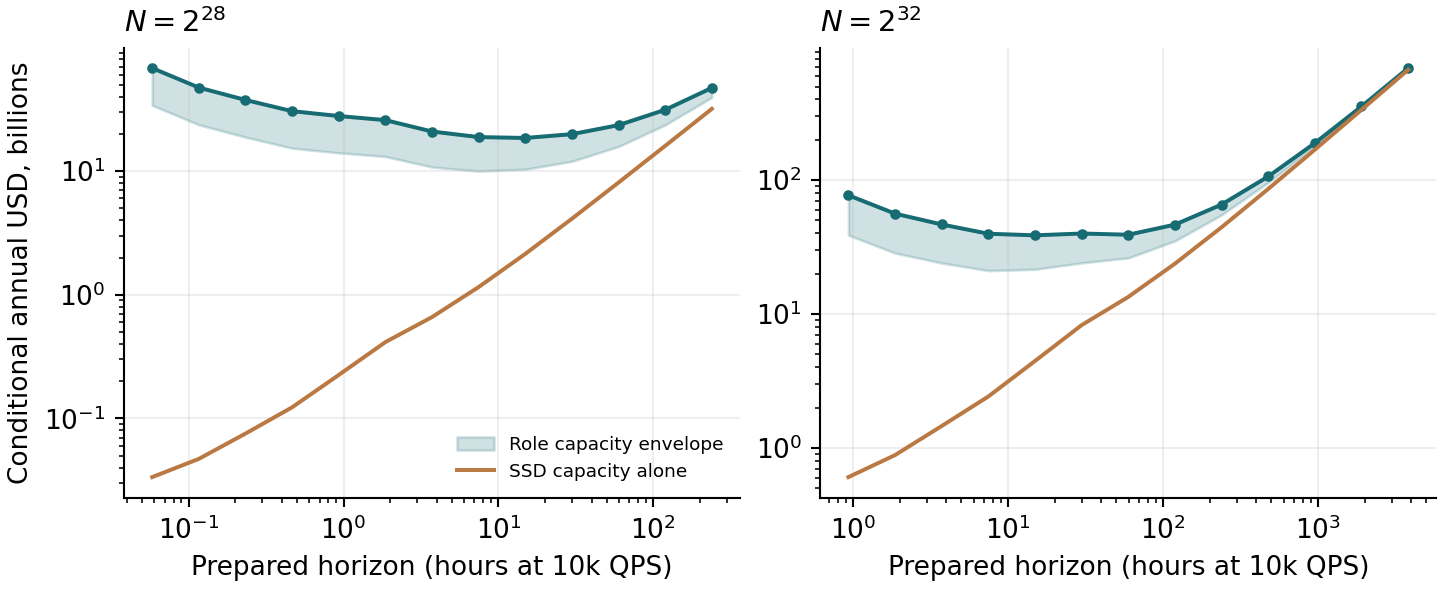
\includegraphics[width=\linewidth]{results/garbled_epoch_cost.png}
\end{center}
\textbf{Shorter epochs are not a solved free refresh.} Re-inputting existing
state pays for encoding; it does not compute a valid jointly hidden layout,
sample and validate private routing controls, or transfer a live state securely
to the next garbling. The two-party source knows controls at its sole garbler;
that role cannot simply be assigned to one possibly corrupted party here.
Also, the cited multiparty theorem uses static corruptions and standalone
function evaluation. Continuously injecting new, possibly adaptive external
client requests through an epoch needs a service-security argument. Internal
RAM adaptivity alone does not establish that API. These integration assumptions
apply at every horizon, including the reference.

\subsection{Sensitivity and comparison with interactive MPC}
\begin{center}\small\begin{tabularx}{\linewidth}{Xrr}\toprule
Change from the $T=2N$ reference & $N=2^{28}$ & $N=2^{32}$\\\midrule
Printed multiplication algebra & \$10.03--17.92B & \$54.68--64.92B \\
Additional correlation traffic: +25\% of prep. & \$12.33--22.52B & \$57.66--70.88B \\
Additional correlation traffic: +100\% of prep. & \$18.33--34.52B & \$65.45--86.46B \\
One complete epoch retained & \$9.26--17.45B & \$32.85--43.47B \\
Ten independent states, two epochs each & \$29.59--37.78B & \$455.07--465.70B \\
Compute two SHA3 hashes inside the circuit & \$10.94--19.62B & \$57.59--68.70B \\
Routing-only initialization allowance & \$12.78--22.91B & \$66.68--79.54B \\
All inter-party bytes cross AZs & \$657.09--665.28B & \$894.27--904.89B \\
\bottomrule\end{tabularx}\end{center}
Each row changes one assumption. The routing-only allowance applies a padded
Bene\v{s} permutation to every tree's physical slots with block width
$w+2h+1$: for $K$ padded slots, it charges $(K/2)(2\log_2 K-1)$ secret switches,
one AND per moved bit per switch, plus encoding the supplied control bits.
It excludes generation and verification of valid controls. Thus it is a concrete additional kernel, not a complete setup
budget. Ten states multiply SSD capacity while sharing the aggregate 10k QPS;
they do not multiply the same query traffic by ten. A one-epoch policy halves
retention, not recurring production cost. Cross-AZ traffic charges both billed
endpoints once per transmitted byte, at \$0.02/decimal GB in total.

The interactive reference costs \$2.33B/\$5.16B per year at the two sizes, with
modeled mean latencies 4.77/3.97 seconds. Its resource bottleneck is local
arithmetic, mostly online work under the baseline phase attribution; at $2^{32}$ RAM capacity also forces additional
machines. The garbled model instead gives a network/SSD resource envelope under
the user-specified network bottleneck, with costly recurring offline production.
We do not claim a five-second garbled-service latency without an evaluation and
scheduling benchmark. Both models include ten parties and sustainable repeated
query work, but their CPU assumptions and replica policies differ. These dollar
figures do not establish a universal protocol ranking.

For the proposal, retain interactive arithmetic compilation as the working
direction and state the concrete benchmark milestones. Neither this garbled
construction nor the unimplemented all-arithmetic reference currently supports
a low-cost production commitment. A tighter garbled estimate requires finite
malicious correlation costs, a joint initialization/renewal implementation,
reactive input handling, a concrete party traffic graph, and measured local
evaluation, including any representation adapters. SSD streaming and independent-state scheduling are additional
optimization opportunities rather than assumed free savings.


\section{Reproduction and next decision}
From the repository root:
\begin{verbatim}
python -m mpc_cost.run --full
python -m mpc_cost.compare_scans
python -m mpc_cost.run --full `
  --config mpc_cost/data/design_2p32.json `
  --output mpc_cost/results/size_2p32
python -m mpc_cost.compare_scans --results mpc_cost/results/size_2p32
python -m mpc_cost.garbled_cost
python -m unittest discover -s mpc_cost -p "test_*.py" -v
python -m mpc_cost.render_report
\end{verbatim}
Compile \texttt{mpc\_cost/mpc\_oram\_cost\_report.tex} with its working directory
set to \texttt{mpc\_cost}. The program has no runtime dependencies beyond Python's
standard library; generating figures additionally needs Matplotlib and PDF
compilation needs LaTeX. \texttt{README.txt} explains overrides and price refresh.
The backticks above continue a command in PowerShell; elsewhere put its arguments
on one line. The garbled sweep saves \texttt{results/garbled\_ram\_comparison.json}.

The tests validate arithmetic witnesses (comparison, gated decoding, duplicate
updates, Fermat equality), recursive base dimensions, metadata movement, all-party
and replica billing, transfer send-counting, and queue saturation. They do not
validate an unimplemented ORAM security proof or MPC performance.
Additional checks validate both database sizes, finite garbling coefficients,
generated versus visited gate counts, routing-only setup, arbitrary traffic-graph
fleet bounds, framing, SSD-copy scaling and transfer accounting.

Before choosing a proposal budget, benchmark checked scalar batches, long dot
products, mask production, and a complete recursive read with duplicate updates.
Measure online latency and sustainable total resource use separately, then replace
the proxy counts and sweep the parameters again.
\end{document}
